\chapter{Divergencias ultravioletas y la solución supersimétrica}

\lectureoverview{Antes de introducir las matemáticas formales de la supersimetría, debemos precisar cuál es el problema que pretende resolver. Describiremos las divergencias ultravioletas tanto en el espacio de posiciones como en el espacio de momentos, deduciremos mediante análisis dimensional el comportamiento a corta distancia de los propagadores de escalares y fermiones, y estimaremos las correcciones dominantes de un lazo a la masa de un escalar. Un lazo escalar y uno fermiónico tienen la misma dependencia cuadrática del corte, pero signos opuestos. La supersimetría se vuelve convincente cuando nos preguntamos qué principio podría hacer coincidir sus acoplamientos, multiplicidades y masas lo suficiente para que esa cancelación sea estructural y no accidental.}

\section{¿Por qué volver a las divergencias?}

La intención era empezar de inmediato con el formalismo de la supersimetría. Sin embargo, es mejor posponer la abstracción una clase y reconstruir la motivación. La explicación anterior de las divergencias y la renormalización de la masa pasó demasiado rápido, y la supersimetría parecerá una invención matemática arbitraria si antes no vemos con exactitud qué hay que corregir.

Los diagramas de Feynman desempeñan dos funciones estrechamente relacionadas en la física de partículas. La más conocida es organizar las amplitudes de dispersión. Especificamos las partículas entrantes y salientes, y sumamos las amplitudes representadas por todos los diagramas del orden requerido. También organizan la construcción de un \emph{Lagrangiano efectivo}. Aquí, ``efectivo'' no es un elogio que signifique especialmente exitoso. Significa que la descripción es aproximada: se han eliminado o integrado los detalles inaccesibles a corta distancia, y su influencia queda codificada en los parámetros e interacciones restantes.

Toda descripción de este tipo tiene un intervalo de validez. Podemos especificarlo mediante la distancia mínima en la que aún es fiable, denotada aquí por \(\delta\), o mediante el momento máximo fiable,
\begin{equation}
\Lambda\sim \delta^{-1}.
\end{equation}
Los dos cortes no son supuestos independientes. Son descripciones duales de Fourier del mismo límite ultravioleta.

\section{Un propagador, dos descripciones}

El propagador es la amplitud de crear o insertar una partícula en un punto del espacio-tiempo y eliminarla o detectarla en otro. Sean los dos puntos \(x^\mu\) y \(y^\mu\), y escribamos su separación como
\begin{equation}
\Delta^\mu=y^\mu-x^\mu.
\end{equation}
Reservamos el símbolo en minúscula \(\delta\) para el corte, a fin de no confundir la separación con el regulador.

La invariancia traslacional implica que un propagador libre depende de \(x\) y \(y\) únicamente a través de \(\Delta\). El mismo objeto puede transformarse de Fourier:
\begin{equation}
G(\Delta)
=\int\frac{d^4k}{(2\pi)^4}\,e^{-ik\cdot\Delta}\,\widetilde G(k).
\end{equation}

Cuando se pregunta a la clase ``¿cuáles son las variables conjugadas de Fourier de la posición?'', la respuesta es el momento. Por consiguiente, la descripción de un lazo en el espacio de posiciones como un propagador que vuelve a su punto de partida equivale a describirlo en el espacio de momentos como una integral sobre todos los momentos que pueden circular por el lazo. Las reglas en el espacio de momentos exigen imponer la conservación del momento en cada vértice; el espacio de posiciones hace más transparente el argumento actual de conteo de potencias.

Esta equivalencia permite identificar el problema ultravioleta antes de hacer ningún cálculo. En el espacio de posiciones, un lazo explora el límite de puntos coincidentes \(\Delta\to0\). En el espacio de momentos, explora el límite \(|k|\to\infty\). Un momento grande corresponde a una longitud de onda corta, así que una singularidad a corta distancia y una divergencia a momentos altos son el mismo fenómeno expresado en coordenadas distintas.

La clase considera las clases de espín más sencillas: campos escalares, campos fermiónicos y, como trasfondo, campos de gauge. Los escalares tienen espín cero y se representan mediante un campo de una componente \(\phi(x)\). Cuando se grabó la clase, en 2010, aún no se había descubierto el Higgs y se lo describía como el principal escalar esperado en la física de partículas. Ese contexto histórico explica la expresión jocosa ``higgly-wiggly'': el campo era de gran interés físico, pero todavía no se había establecido experimentalmente.

Para un campo escalar real, el propagador puede escribirse esquemáticamente como
\begin{equation}
G_\phi(x,y)=\expect{0|T\!\left\{\phi(x)\phi(y)\right\}|0}
=G_\phi(\Delta).
\end{equation}
La convención de ordenamiento temporal y la normalización no afectarán nuestro conteo de potencias. Lo importante es que las dos inserciones del campo describen su creación en un punto y su aniquilación en el otro.

\begin{classroomqa}
\audiencequestion{¿\(x\) y \(y\) son posiciones en el espacio o en el espacio-tiempo? \lecturetimestamp{00:09:31}}
\lecturerresponse{Son puntos del espacio-tiempo. Cada uno es un cuadrivector. Por tanto, el propagador depende de su separación cuatridimensional y, en un vacío invariante de Lorentz, del intervalo invariante correspondiente.}
\end{classroomqa}

Una partícula de espín un medio se describe mediante un campo de Dirac \(\psi_i(x)\). El índice \(i\) es un índice espinorial, no una componente espacial, así que el propagador es una matriz:
\begin{equation}
S_{ij}(x,y)=\expect{0|T\!\left\{\psi_i(x)\bar\psi_j(y)\right\}|0}
=S_{ij}(\Delta).
\end{equation}

Una pregunta a la clase permite precisar el número de componentes: un campo de Dirac en cuatro dimensiones tiene cuatro componentes complejas. Un campo de Weyl sin masa puede describirse con dos componentes complejas, de modo que los campos levógiros y dextrógiros pueden tratarse por separado. Para el argumento dimensional actual, solo importa que exista una estructura matricial espinorial.

Como \(S_{ij}\) es una matriz \(4\times4\), puede desarrollarse en la base de las matrices de Dirac. Al principio omitiremos esos índices y los restituiremos cuando sean necesarios. No afirmamos que la estructura matricial esté ausente; la simplificamos deliberadamente mientras establecemos la ley de potencias ultravioletas.

\begin{classroomqa}
\audiencequestion{¿Cuándo debe aparecer el campo conjugado o adjunto en un propagador? \lecturetimestamp{00:14:06}}
\lecturerresponse{Para un escalar neutro real en esta descripción esquemática, el mismo campo contiene operadores de creación y aniquilación, así que no hace falta un campo adjunto distinto. Para un campo cargado, hay que distinguir los operadores de partículas y antipartículas. Por tanto, \(\psi\), \(\psi^\dagger\) y, de forma covariante, \(\bar\psi=\psi^\dagger\gamma^0\), desempeñan papeles distintos en el caso del electrón.}
\end{classroomqa}

La partícula física de Higgs es neutra, aunque el campo de Higgs subyacente del Modelo Estándar es un doblete electrodébil. La clase toma como modelo local el escalar neutro real; esa simplificación basta para la estimación ultravioleta.\editorialnote{Esta distinción evita confundir el ejemplo esquemático del escalar real con una descripción completa del multiplete de Higgs electrodébil.}

\section{Unidades naturales y dimensión de un campo escalar}

Tomemos \(\hbar=c=1\). La longitud y el tiempo tienen entonces las mismas unidades, mientras que la energía, la masa y el momento tienen unidades de longitud inversa:
\begin{equation}
[m]=[E]=[p]=L^{-1}.
\end{equation}
La acción aparece en la fase \(e^{iS}\), así que es adimensional. Una acción escalar representativa en cuatro dimensiones espacio-temporales es
\begin{equation}
S_\phi=\int d^4x\left[
\frac12\partial_\mu\phi\,\partial^\mu\phi
-\frac12m^2\phi^2
-\frac{\lambda}{4!}\phi^4
+\cdots\right].
\end{equation}
Los factores convencionales \(1/2\) y \(1/4!\) no afectan al análisis dimensional.

Empecemos por el término cinético. Como \([d^4x]=L^4\) y \([\partial_\mu]=L^{-1}\), la condición de adimensionalidad implica
\begin{align}
1
&=L^4\left(L^{-1}[\phi]\right)^2,\\
[\phi]&=L^{-1}.
\end{align}
El término de masa sirve de comprobación:
\begin{equation}
L^4[m^2][\phi^2]
=L^4L^{-2}L^{-2}=1.
\end{equation}

La siguiente pregunta a la clase es cuál es la dimensión del acoplamiento cuártico. En cuatro dimensiones espacio-temporales es adimensional:
\begin{equation}
L^4[\lambda][\phi]^4=L^4[\lambda]L^{-4}=1
\quad\Longrightarrow\quad [\lambda]=L^0.
\end{equation}
Esto hace que la interacción \(\phi^4\) sea especial en cuatro dimensiones. Las dimensiones de \(\phi^6\) y de las interacciones de orden superior se obtienen con la misma regla, pero sus acoplamientos llevan potencias negativas de la masa y, por tanto, indican un papel más restringido dentro de una teoría efectiva.

Las dimensiones de los campos ya nos indican qué interacciones pueden aparecer con coeficientes adimensionales. El mismo método determinará los dos propagadores y el acoplamiento de Yukawa sin evaluar una integral de Feynman detallada.

\section{El propagador escalar a corta distancia}

Consideremos primero un escalar sin masa. No hay una escala intrínseca, así que la única escala disponible es la separación \(\Delta\). La invariancia traslacional deja únicamente \(\Delta\), la invariancia de Lorentz reduce la dependencia a su magnitud invariante, y el producto de dos campos escalares tiene dimensión \(L^{-2}\). Salvo una constante numérica,
\begin{equation}
G_0(\Delta)\sim\frac{1}{\Delta^2}.
\end{equation}
El razonamiento dimensional por sí solo no permite fijar factores como \(4\pi^2\).

La masa introduce la longitud de Compton \(m^{-1}\). Su efecto se entiende mejor a partir de la relación de dispersión
\begin{equation}
E=\sqrt{\bm p^{,2}+m^2},
\qquad
E=|\bm p|\quad(m=0).
\end{equation}
Cuando \(|\bm p|\gg m\), la masa es despreciable. Como los momentos altos sondean distancias cortas, el propagador masivo debe aproximarse al comportamiento sin masa \(1/\Delta^2\) cuando \(\Delta\to0\). A distancias mucho mayores que \(m^{-1}\), la propagación queda suprimida. La clase representa este hecho esquemáticamente mediante
\begin{equation}
G_m(\Delta)\sim \frac{e^{-m|\Delta|}}{\Delta^2}.
\end{equation}
Esta no es, deliberadamente, una fórmula exacta. En el espacio euclídeo cuatridimensional, el propagador libre exacto es proporcional a \(mK_1(mr)/r\), con \(r=|\Delta|\); presenta la misma singularidad ultravioleta \(1/r^2\) y una caída exponencial a grandes distancias acompañada por un prefactor de ley de potencias.\editorialnote{La expresión con la función de Bessel proporciona la forma precisa estándar que completa la exponencial esquemática de la clase; no hace falta para el argumento de conteo de potencias.}

La lección fundamental es sencilla: la masa suaviza la propagación a grandes distancias, pero no corrige la singularidad en puntos coincidentes. Lo bastante cerca de un punto, cualquier masa finita se vuelve irrelevante.

\section{El tadpole escalar y el ajuste fino}

La interacción cuártica \(\lambda\phi^4\) produce un vértice de cuatro líneas. Unamos dos de sus patas entre sí y dejemos dos patas escalares externas. El diagrama de tadpole resultante corrige el coeficiente de \(\phi^2\) y, por tanto, la masa al cuadrado del escalar.

El fotograma conservado capta la transición exacta del análisis dimensional a esta corrección de lazo. A la izquierda permanece la relación de dispersión; a la derecha aún se ven parcialmente la acción escalar y la dimensión del campo, y en el centro acaba de aparecer el pequeño tadpole.

\begin{figure}[H]
\centering
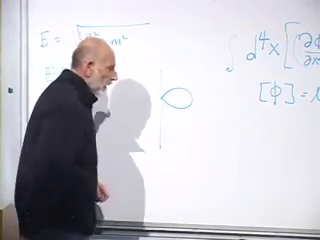
\includegraphics[width=0.72\textwidth]{lecture_03_figure_02.png}
\lectureframe{00:28:30.560}

\medskip
\begin{tikzpicture}[line width=0.8pt,scale=1.0]
  \draw[dashed] (-2.6,0) -- (0,0) -- (2.6,0);
  \fill (0,0) circle (0.055);
  \draw (0,0) .. controls (-0.85,0.7) and (-0.85,1.6) .. (0,1.6)
                .. controls (0.85,1.6) and (0.85,0.7) .. (0,0);
\end{tikzpicture}
\caption{La pizarra durante la transición a la autoenergía escalar, seguida de un redibujo esquemático prudente de la topología del tadpole. La captura muestra claramente el lazo, las fórmulas relativista y sin masa de la energía, y una parte de la acción; no se afirma que los coeficientes y rótulos ocultos sean visibles.}
\end{figure}

En el vértice, el escalar puede absorberse y reemitirse mientras las otras dos patas se propagan desde el punto de vuelta a sí mismo. Salvo factores numéricos y combinatorios, la corrección es
\begin{equation}
\delta m_\phi^2\sim \lambda G_\phi(0).
\end{equation}
El propagador en puntos coincidentes es infinito en la aproximación del continuo. Una teoría efectiva no pretende ser válida a distancias arbitrariamente cortas, así que imponemos \(|\Delta|\geq\delta\). Entonces,
\begin{equation}
G_\phi(0)\longrightarrow G_\phi(\delta)sim\frac{1}{\delta^2},
\qquad
\delta m_\phi^2\sim\frac{\lambda}{\delta^2}sim\lambda\Lambda^2.
\end{equation}
Se llama cuadrática a la divergencia porque contiene dos potencias del corte de momento. La integración en el espacio de momentos lleva a la misma conclusión: la contribución excesiva procede de momentos de lazo arbitrariamente grandes. Que la escala mínima quede determinada finalmente por la gran unificación, la gravedad cuántica o algo aún inimaginado no cambia el diagnóstico de la teoría efectiva.

Este es un problema de ajuste fino. Si \(\delta\) es extremadamente pequeño y \(\lambda\) no es extraordinariamente diminuto, la corrección radiativa es mucho mayor que la masa al cuadrado del escalar observada a bajas energías. Por tanto, el coeficiente desnudo y la corrección de lazo deben cancelarse hasta un número implausible de cifras:
\begin{equation}
m_{\mathrm{physical}}^2
=m_{\mathrm{bare}}^2+\delta m_\phi^2.
\end{equation}
El propagador masivo no resuelve la situación. A las distancias responsables de la divergencia, \(e^{-m|\Delta|}\simeq1\). El lazo ultravioleta ha dejado de depender de la masa mucho antes de alcanzar el corte.

\section{Dimensiones de los fermiones y su propagador}

Repitamos ahora el mismo análisis dimensional para un fermión de Dirac. Su acción libre es
\begin{equation}
S_\psi=\int d^4x\,
\bar\psi\left(i\gamma^\mu\partial_\mu-m\right)\psi.
\end{equation}
Las matrices gamma son numéricas y adimensionales. El término cinético contiene una sola derivada, así que
\begin{align}
1
&=L^4[\bar\psi]L^{-1}[\psi],\\
[\psi]=[\bar\psi]&=L^{-3/2}.
\end{align}
Las potencias semienteras no deberían alarmarnos: los fermiones introducen mitades en muchos lugares.

\begin{classroomqa}
\audiencequestion{¿No sería más fácil deducir \([\psi]\) a partir del término de masa? \lecturetimestamp{00:36:02}}
\lecturerresponse{Sí. El término de masa da \(L^4L^{-1}[\bar\psi\psi]=1\), de donde se obtiene \([\bar\psi\psi]=L^{-3}\) y \([\psi]=L^{-3/2}\). Primero usamos la derivación a partir del término cinético porque sigue siendo válida en la teoría sin masa y muestra por qué la masa del fermión aparece como \(m\), y no como \(m^2\).}
\end{classroomqa}

Dos campos fermiónicos tienen dimensión \(L^{-3}\), así que la abreviatura dimensional de la clase para el propagador sin masa es
\begin{equation}
S(\Delta)\sim\frac{1}{|\Delta|^3}.
\end{equation}
Al restituir su estructura matricial, se obtiene el numerador más preciso que exige la covariancia de Lorentz:
\begin{equation}
S_{ij}(\Delta)
\propto
\frac{\left(\gamma_\mu\Delta^\mu\right)_{ij}}
{\left(\Delta^2\right)^2}.
\end{equation}
El numerador añade una potencia de longitud, y el denominador contiene, por tanto, cuatro potencias del intervalo; la dimensión neta sigue siendo \(L^{-3}\). Al igual que en el caso escalar, la masa del fermión suprime el propagador a grandes separaciones, pero deja inalterado este escalamiento a corta distancia.

\section{Por qué un lazo fermiónico cerrado es negativo}

Ahora podemos preguntarnos si un diagrama fermiónico podría cancelar la autoenergía bosónica problemática. El tadpole escalar tiene signo positivo, salvo factores numéricos positivos como potencias de \(\pi\) y coeficientes combinatorios. Un lazo fermiónico cerrado tiene el signo opuesto.

\begin{classroomqa}
\audiencequestion{¿El signo menos del lazo fermiónico está relacionado con la explicación anterior de una rotación completa? \lecturetimestamp{00:40:21}}
\lecturerresponse{Forma parte de la misma estructura de signos fermiónica, pero aquí la demostración útil se basa en la antisimetría de intercambio, no en la orientación geométrica del lazo. Cortemos dos lazos, intercambiemos las partículas idénticas y volvamos a conectarlos. El intercambio convierte dos lazos en uno y aporta un signo menos solo para los fermiones.}
\end{classroomqa}

Vale la pena desarrollar el argumento completo. Supongamos que un diagrama de un lazo tiene signo \(\sigma\), positivo o negativo. Dos lazos idénticos y desconectados tienen signo
\begin{equation}
\sigma^2=+1.
\end{equation}
Cortemos simultáneamente ambos lazos. Ahora tenemos dos partículas idénticas que se propagan entre los cortes. Su función de onda ordinaria de dos partículas es simétrica para los bosones y antisimétrica para los fermiones:
\begin{align}
\Psi_B(x_1,x_2)&=+\Psi_B(x_2,x_1),\\
\Psi_F(x_1,x_2)&=-\Psi_F(x_2,x_1).
\end{align}
La antisimetría también explica el principio de exclusión de Pauli: si ambos fermiones ocupan el mismo estado, el intercambio no cambia nada físicamente, pero debe invertir la función de onda, que por tanto ha de anularse.

Volvamos a conectar las líneas cortadas después de intercambiar las dos partículas. Topológicamente, los dos lazos se han convertido en uno. La amplitud de los dos lazos sin intercambiar era positiva. El intercambio la deja positiva para los bosones y cambia su signo para los fermiones. Por tanto,
\begin{equation}
\begin{aligned}
\operatorname{sign}(\text{closed boson loop})&=+1,\\
\operatorname{sign}(\text{closed fermion loop})&=-1.
\end{aligned}
\end{equation}
La conclusión es general: cada lazo fermiónico cerrado independiente aporta un factor de \(-1\).

\section{El lazo de Yukawa}

Volvamos a la masa del escalar. Un bosón no puede convertirse en un solo fermión porque cambiaría la paridad del número fermiónico. La corrección fermiónica más sencilla consiste en que el escalar se divida en un par de fermión y antifermión, que se propagan formando un lazo y vuelven a recombinarse. La interacción es un acoplamiento de Yukawa,
\begin{equation}
\mathcal L_Y=-g\phi\bar\psi\psi.
\end{equation}
En el caso del Higgs, los fermiones pueden ser quarks o leptones. Hay dos puntos de interacción y, por tanto, dos factores de \(g\).

El tadpole escalar implicaba un solo punto, cuya posición global podía fijarse porque la invariancia traslacional solo aporta el volumen del espacio-tiempo. El lazo de Yukawa implica dos puntos. Podemos fijar uno de ellos o, de forma equivalente, fijar la posición media de ambos, pero debemos integrar sobre su separación relativa \(\Delta\). Cada propagador fermiónico aporta el factor de corta distancia \(1/|\Delta|^3\), así que
\begin{equation}
\delta m_{\phi,F}^2
\sim
-g^2\int_{|\Delta|\geq\delta}d^4\Delta\,
\frac{1}{|\Delta|^6}.
\end{equation}

Una vez escritos los dos propagadores, la integral sobre la separación y los dos acoplamientos, se pide a la clase un último factor. La respuesta es el signo menos. Los dos propagadores se cierran formando un lazo fermiónico, así que la integral de corta distancia, positiva en todo lo demás, queda multiplicada por \(-1\).

El análisis dimensional ya determina la divergencia. La medida \(d^4\Delta\) aporta cuatro potencias de longitud, hay seis en el denominador y la única escala de longitud restante es el corte:
\begin{equation}
\int_{|\Delta|\geq\delta}
\frac{d^4\Delta}{|\Delta|^6}
\sim\frac{1}{\delta^2}.
\end{equation}
Esto puede hacerse explícito con coordenadas radiales euclídeas en cuatro dimensiones:
\begin{equation}
\int_{\delta}^{R}d^4\Delta\,\frac{1}{|\Delta|^6}
=2\pi^2\int_{\delta}^{R}dr\,\frac{r^3}{r^6}
=\pi^2\left(\frac{1}{\delta^2}-\frac{1}{R^2}\right).
\end{equation}
Las trazas espinoriales y las normalizaciones de los propagadores modifican el coeficiente, pero no la dependencia cuadrática del corte.\editorialnote{La integral radial es una versión explícita estándar de la estimación dimensional hecha en la clase. Está escrita en términos de la distancia euclídea, donde la positividad y el conteo de potencias ultravioletas son transparentes.}

\begin{classroomqa}
\audiencequestion{¿Cambiaría el signo invertir o elegir otros límites de integración? \lecturetimestamp{00:51:06}}
\lecturerresponse{No. No se trata de una integral unidimensional orientada cuyos límites generen el signo físico. Es una integral sobre cuatro componentes o, de manera más clara, sobre una medida radial positiva. Su contribución ultravioleta es positiva. La contribución negativa procede únicamente del lazo fermiónico cerrado.}
\end{classroomqa}

\begin{classroomqa}
\audiencequestion{¿Cuál es la dimensión del acoplamiento de Yukawa \(g\)? \lecturetimestamp{00:51:51}}
\lecturerresponse{Es adimensional en cuatro dimensiones. Como \([\phi]=L^{-1}\) y \([\bar\psi\psi]=L^{-3}\), el producto \(\phi\bar\psi\psi\) tiene dimensión \(L^{-4}\), que queda exactamente compensada por \(d^4x\).}
\end{classroomqa}

La corrección fermiónica dominante es, por tanto,
\begin{equation}
\delta m_{\phi,F}^2
\sim -C_F\frac{g^2}{\delta^2}
=-C_Fg^2\Lambda^2,
\end{equation}
donde \(C_F>0\) contiene factores numéricos, espinoriales y de multiplicidad. El lazo escalar tiene la forma correspondiente
\begin{equation}
\delta m_{\phi,B}^2
\sim+C_B\frac{\lambda}{\delta^2}
=+C_B\lambda\Lambda^2.
\end{equation}
Aún no hemos resuelto el problema del ajuste fino, pero hemos encontrado algo indispensable: una contribución con el mismo grado de divergencia ultravioleta y signo opuesto.

\section{Qué exige la cancelación}

Sería una coincidencia extraordinaria que acoplamientos sin relación entre sí satisficieran
\begin{equation}
C_B\lambda=C_Fg^2
\end{equation}
con la precisión exacta que exige una gran jerarquía de escalas. La clase lo abrevia como \(g^2=\lambda\), omitiendo factores dependientes de las convenciones y de las multiplicidades. Una solución genuina requiere una estructura matemática que imponga la relación, no que se limite a permitirla.

Esa es la motivación de la supersimetría. La supersimetría relaciona bosones y fermiones y restringe sus acoplamientos a combinaciones que cancelan muchos términos divergentes que, de otro modo, serían problemáticos. La cancelación se repite entonces en todos los diagramas porque se deriva de una simetría, no de un ajuste de parámetros hecho lazo a lazo.

La coincidencia de masas también importa. Si las masas del bosón y del fermión son idénticas, sus propagadores completos pueden emparejarse con mayor precisión. Si las masas difieren ligeramente, las respuestas finitas completas no se cancelan de manera exacta, porque los propagadores difieren a distancias comparables con sus longitudes de Compton. Sin embargo, sus comportamientos asintóticos comunes a corta distancia pueden cancelar la parte divergente:
\begin{equation}
\mathcal I_B(\Delta)-\mathcal I_F(\Delta)
\quad\hbox{may be finite as}\quad \Delta\to0,
\end{equation}
donde \(\mathcal I_B\) y \(\mathcal I_F\) denotan los integrandos completos de los lazos bosónico y fermiónico, una vez incluidos los vértices, los numeradores y las multiplicidades. No se restan directamente los propagadores, que tienen dimensiones distintas. Aunque se cancelen los términos ultravioletas, puede quedar un residuo finito. Esto abre la posibilidad de una supersimetría aproximada o rota. La igualdad exacta produce la cancelación más limpia; una ruptura suficientemente controlada aún puede eliminar la catástrofe ultravioleta y dejar desdoblamientos de masa observables.

Así pues, hemos llegado a la supersimetría sin escribir todavía su álgebra. La cadena de razonamiento está completa:
\begin{equation}
\begin{gathered}
G_\phi(\Delta)\sim \Delta^{-2},
\qquad
\delta m_{\phi,B}^2\sim+C_B\lambda\Lambda^2,\\[0.4em]
S_\psi(\Delta)\sim \Delta^{-3},
\qquad
\delta m_{\phi,F}^2\sim-C_Fg^2\Lambda^2,\\[0.4em]
\text{symmetry-enforced matching}\\
\Longrightarrow\quad
\text{quadratic divergences cancel}.
\end{gathered}
\end{equation}
La tarea siguiente es entender el principio de simetría abstracto que impone esas relaciones y examinar ejemplos concretos de cómo actúa.